\documentclass[12pt]{article}

\usepackage{sbc-template}

\usepackage{graphicx,url}

%\usepackage[brazil]{babel}   
\usepackage[latin1]{inputenc}  

     
\sloppy

\title{Comparison of Methods of Noise Classification}

\author{Antonio Nascimento\inst{1}, Felipe de S. Farias\inst{1}, Marilia Alves \inst{2}}


\address{Programa de Pos-Graduacao em Engenharia de Defesa \\ Instituto Militar de Engenharia (IME)\\
\nextinstitute
  Programa de Pos-Graduacao em Engenharia Eletrica \\ Instituto Militar de Engenharia (IME)
\nextinstitute
  \email{\{antonio.nascimento,felipe.farias,marilia.alves\}@ime.eb.br}
}

\begin{document} 

\maketitle

\begin{abstract}

%This is the paper model for SBC conferences. I made some instructions so we can use it to write our own paper. It contains a suggestion of placement of the sections. 

Ok here we make the abstract. Needless to say it comes last. Should have max 10 lines.

\end{abstract}
     


\section{Introduction} \label{sec:intro}


%I took some liberties in the sketch Nascimento gave us in the Telegram group, combining with this paper \cite{nakagawa2012speaker} to come up with this model you're seeing. Initially, this Section describes the problem we are attempting to solve. We have to describe the problem many audio signal processing tasks face when performed in noisy conditions. References are much appreciated.

%After that, we should write some kind of small version of the next sections. Do it ONLY after writing all the other parts. Each paragraph in the other sections become some lines here.

Many Acoustic Signal Processing (ASP) tasks are performed in noisy conditions. The presence of noise, additive or otherwise, decreases the performance of those tasks, be it speaker recognition \cite{ming2007robust}, emotion recognition \cite{schuller2010cross}, source localization \cite{benesty2000adaptive} or speech recognition \cite{friesen2001speech}. Thus, it is imperative to study noise so we can better assess how it affects ASP tasks and how we can deal with it. Automatic classification of types of noise is an important part of this study, since the knowledge of the kind of noise present in a given situation is useful knowledge to better treat it \cite{may2012noise}.

There is extensive previous work in the field of audio classification. There is great variety in the methods used to perform this task, such as statistical methods \cite{dal1988acoustic,peltonen2002computational}, methods using stochastical knowledge such as \textit{Hidden Markov Models} (HMM) \cite{ma2003context}, using neural networks \cite{beritelli2005adaptive} and support vector machines \cite{cumani2012analysis}. There is variety also in the applications sought, such as speaker recognition \cite{kinnunen2010overview,murty2006combining,farrell1994speaker}, acoustic scene recognition \cite{piczak2015environmental,barchiesi2015acoustic} or animal species recognition \cite{somervuo2006parametric,lee2008automatic}. The noise classification is different only in application, but can be performed using any method used for audio classification \cite{beritelli2007adaptive,ma2006acoustic}.

This work proposes to evaluate the performance of four common methods used in audio classification in the specific task of classify noise. To this end, we implement those methods in the same set of audio files containing different types of noise. These files are taken from the NOISEX database \cite{varga1993assessment}, a database comprised of audios of 15 types of noise. The evaluation follows these steps: The extraction of attributes of each audio file, construction of the models according to each method, classification and evaluation of the results. The methods compared are the Neural Network, Gaussian Mixture Model, Support Vector Machines and K-means.

The remainder of this paper is organized as follows. Section \ref{class} introduces the task of noise classification, as long as the methods used in this paper. Section \ref{exp} describes the experiments performed and the results obtained and, finally, in Section \ref{conc} we present our conclusions about the results found, as long as the future works.

\section{Noise Classification} \label{class}

%In this section we should describe the audio classification task and how it applies to our specific problem, the noise classification.

%Additionally, we have to describe each method we use, in subsections.

\subsection{Extraction of Audio Attributes} \label{class:audioatt}

The first step towards classification is the extraction of attributes from the data that are useful for the classification algorithms. In this Section we present two of the most widely used in the literature, the Linear Predictive Coefficient \cite{Rabiner:1993:FSR:153687} and the Mel-Frequency Cepstral Coefficient (MFCC) \cite{xu2005automatic}. In this work, we will use the MFCC to represent our audios.

\subsubsection{Linear Predictive Coefficient (LPC)}\label{class:lpc}

In the Linear Predictive analysis of audio, the audio is divided into frames of the same size, usually 20ms, and each frame is predicted as the linear weighted sum of the \textit{n} previous frames, there \textit{n} represents the order of the prediction \cite{Rabiner:1993:FSR:153687}. 

\begin{equation}
	\hat{s} = \sum_{k=0}^{n} \alpha_ks(n-k)
	\label{eq:lpc}
\end{equation}


The difference between the prediction and the actual values of the frame is computed as error. The coefficients $\alpha_k$ are obtained minimizing the prediction error through the least squares minimization.


\subsubsection{Mel-Frequency Cepstral Coefficient (MFCC)} \label{class:mfcc}

The Mel-Frequency cepstrum is efficient in modeling pitch and frequency content of audio signals. It yields better results when coding audio for in classification tasks than the LPC \cite{li2001classification}.

In the mel-cepstral analysis, the audio signal is filtered by \textit{K} bandpass filters, which have constant mel-frequency interval and cover the $0-4000$Hz frequency range. The MFCCs are calculated by the following equation:

\begin{equation}
	c_n = \sqrt{\frac{2}{K}} \sum_{k=1}^{K} (\log S_k) \cos [n(k-0.5)\pi/K]
	\label{eq:mfcc}
\end{equation}

In which $c_n$ is the coefficient for the $n^{th}$ frame and $S_k, k=(1,2,...,K)$ are the output of each bandpass filter.

In this work, we used $K = 13$, and the $\delta_n = c_n - c_{n-1}$ and $\delta\delta = \delta_n - \delta_{n-1} $ coefficients were calculated, thus rendering 39 coefficients by frame.

\subsection{Classification Methods} \label{class:meth}

\subsubsection{K-means} \label{class:kmeans}

This is a method used in summarization. Didn't find references.

\subsubsection{Gaussian Mixture Models (GMM)} \label{class:gmm}

%This section describes the use of Gaussian mixture models (GMM) in the task of noise representation and classification. Here is a good journal article for further reference \cite{reynolds1995robust}.

The GMM is used based on the knowledge that a set of acoustic signal classes can be represented by it's component densities \cite{reynolds1995robust}. The GMM is a weighted sum of $K$ component densities, given by:

\begin{equation}
	p(\vec{x}|\lambda) = \sum_{k=1}^{K} p_kb_k(\vec{x})
	\label{eq:gmm}
\end{equation}

Where $\vec{x}$ is a random vector representing our input signal, $K$ is the number of components of the signal, $p_k, k = 1,...,K$ are the mixture weights and $b_k(\vec{x}), k = 1,...,K$ are the component densities.

Each class is represented by it's model $\lambda$:

\begin{equation}
	\lambda = \{ p_k, \vec{\mu}_k, \sum k \}, k = 1,...,K
	\label{eq:lambda}
\end{equation}

Where $\vec{\mu}_k$ is the mean and $\sum k$ is the covariance matrix of each component density $b_k(\vec{x})$.



\subsubsection{Support Vector Machines (SVM)} \label{class:svm}


The SVM is a machine learning technique that has successfully been used in pattern recognition tasks, such as audio classification \cite{dhanalakshmi2009classification}. The basic idea of this technique is to estimate the hyperplane that better separates a group of data \cite{cumani2012analysis}. The hyperplane can be linear or be created using a kernel function to better do the separation.

There are two distinct phases: in the training phase, the algorithm estimates the best hyperplane, searching for the one that maximizes the distance between the training data of different classes. In the test phase, the classification using the trained hyperplane is performed using different data. This way, we can assess the generalization capacity of the model.

KERNEL QUADRATICO UTILIZADO


\subsubsection{Neural Network} \label{class:nn}

%One or two paragraphs should do. Don't forget the proper references (like this one \cite{lei2014novel}).

Neural Network is an interconnected group of artificial neurons designed to simulate the functionality of a brain. It is organized in layers: the input layer, the hidden layer and the output layer. Each neuron has it's own weight and a activation function \cite{wu2007leaf}. 

In the classification task, the weights of the neurons are updated by training the network with labeled data, until the network can yield the expected result in the output layer.

50 NEURONS UTILIZADOS


\section{Experiments} \label{exp}

%Here we will describe the experiments. It should contain an introductory paragraph containing the purpose of the experiments.

\subsection{Experimental Setup} \label{exp:setup}

%This paragraph should have all the requirements to perform the experiment, including hardware, software and general conditions. Sometimes people put the database here, but i think it will provide greater value if we put it in it's own subsection.

The experiments were performed using MATLAB, using the Neural Network toolbox and the SVM toolbox. They were performed in two separated computers. The K-means and GMM experiments were performed with an Intel-i7 1,8GHz processor, with ram memory of 8GB and Windows10 OS. The Neural Network and SVM experiments were performed with an an Intel-i3 processor, with ram memory of 4GB and Linux OS.

\subsection{Database Description} \label{exp:data}

%Here we describe the NOISEX database. Since it's an important part of this work, we should take our time to properly describe it.

For this work we used the NOISEX database \cite{varga1993assessment}. This database is composed by 15 audio files, one for each of the 15 different classes of noises, which are shown in Table \ref{tab:noisex}. All the audio files are in .wav format, 3 minute and 55 seconds long and they have a bit rate of $319$ kbits per second.

\begin{table}[ht]
	\centering
	\caption{Classes existing in the NOISEX database.}
	\label{tab:noisex}
	\begin{tabular}{lllll}
		\hline
		babble & buccaneer 1 & buccaneer 2 & destroyer engine& destroyer operations room\\
		f16 & factory floor 1 & factory floor 2 & HF channel & leopard\\
		m109 & machine gun & pink noise & volvo & white noise\\
		\hline
	\end{tabular}
\end{table}

\subsection{Cross-Validation} \label{exp:crossv}

The 4-fold cross-validation was performed. The accuracy reported in Table \ref{tab:acc} are the mean of the results in each test. This way, the generalization of each model is better asserted.

\subsection{Results} \label{exp:res}

You may be wondering why have only the 'results' and not the 'experiments' subsection. This is because we already told the reader everything he has to know in the previous sections. Section \ref{class} describes the different methods and Sections \ref{exp:setup} and \ref{exp:data} describe the details of the experiments.


\begin{table}[h]
\centering
\caption{Confusion Matrix for Neural Network}
\label{tab:confusion_nn}
\resizebox{\textwidth}{!}{\begin{tabular}{l||l|l|l|l|l|l|l|l|l|l|l|l|l|l|l}
\hline
& Babble & Bucc 1 & Bucc 2 & Dest Eng & Dest Ops & F16 & Fac 1 & Fac 2 & HFChn & Leop & M109 & MachGun & Pink & Volvo & White \\
\hline
\hline
Babble & 6,5\% & & & & & & 0,1\% & 0,1\% & & & & & & & \\
\hline
Buccaneer 1 & &6,6\% & & & & & & & & & & & & & \\
\hline
Buccaneer 2  & & & 6,7\% & & & & & & & & & & & & \\
\hline
Destroyer Engine  & & & & 6,6\% & & & & & & & & & & & \\
\hline
Destroyer Ops & & & & & 6,5\%& & & & & & & & & & \\
\hline
F16 & & & & & & 6,6\% & & & & & & & & & \\
\hline
Factory 1 & & & & & & & 6,0\% &0,2\% & & & & & 0,1\% & & \\
\hline
Factory 2 & & & & & & & 0,3\%& 6,4\% & & & & & & & \\
\hline
HF Channel & & & & & & & & & 6,7\% & & & & & & \\
\hline
Leopard & & & & & & & & & &6,6\% & & & & & \\
\hline
M109 & & & & & & & & & & &6,6\% & & & & \\
\hline
Machine Gun & & & & & & & & & & & &6,6\% & & & \\
\hline
Pink & & & & & & & 0,2\% & & & & & &6,6\% & & \\
\hline
Volvo & & & & & & & & & & & & & &6,6\% & \\
\hline
White & & & & & & & & & & & & & & & 6,7\%\\
\hline
\end{tabular}}
\end{table}


\begin{table}[ht]
\centering
\caption{Accuracy per class for the methods compared.}
\label{tab:acc}
\begin{tabular}{l|llll}
\hline
Class & K-means & GMM & Neural Network & SVM \\
\hline
Babble & 88,2\% & 98,9\% & 97,5\% &  \\
Bucanneer 1 & 96,6\% & 99,1\% & 99,1\% & \\
Bucanneer 2 & 98,8\% & 99,7\% & 99,8\% & \\
Destroyer Engine & 99,8\% & 99,7\% & 99,7\% & \\
Destroyer Ops & 90,8\% & 96,9\% & 98,3\% &\\
F16 & 95,2\% & 99,10\% & 97,6\% &\\
Factory 1 & 59,3\% & 87,6\% & 92,3\% &\\
Factory 2 & 93,9\% & 95,0\% & 94,7\% &\\
HF Channel & 100,0\% & 100,0\% & 99,9\% &\\
Leopard & 99,1\% & 99,6\% & 99,4\% &\\
M109 & 94,1\% & 99,3\% & 99,3\% &\\
Machine Gun & 7,1\% & 99,5\% & 99,5\% &\\
Pink & 99,7\% & 98,0\% & 96,9\% &\\
Volvo & 90,8\% & 99,4\% & 99,7\% &\\
White & 99,9\% & 99,9\% & 100,0\% &\\
\hline
\textbf{OVERALL} & 89,2\% & 98,0\% & 98,4\% & \\
\hline
\end{tabular}
\end{table}



\section{Conclusions} \label{conc}

Here we conclude the paper. I suck at this, so pls someone do it for me. The one thing I know is that we have to summarize our findings and link it to our problem stated in the introduction, telling the reader whether we were successful or not in the task we proposed in the beginning.

%exemplo de figura

%\begin{figure}[ht]
%\centering
%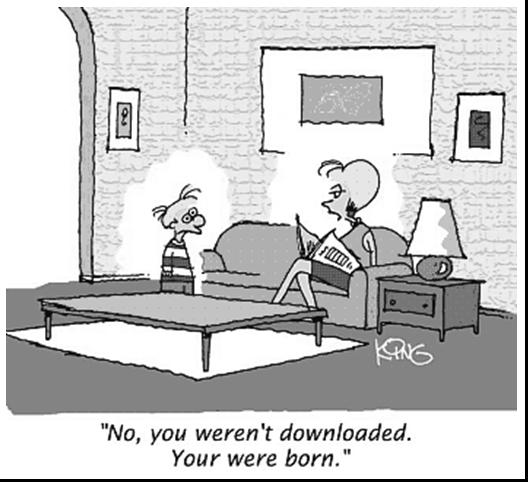
\includegraphics[width=.5\textwidth]{fig1.jpg}
%\caption{A typical figure}
%\label{fig:exampleFig1}
%\end{figure}

%\begin{figure}[ht]
%\centering
%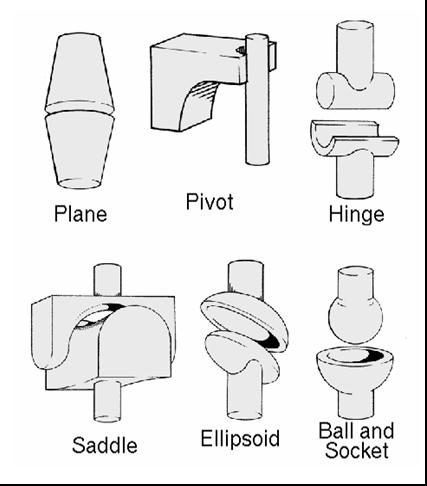
\includegraphics[width=.3\textwidth]{fig2.jpg}
%\caption{This figure is an example of a figure caption taking more than one
%  line and justified considering margins mentioned in %Section~\ref{sec:figs}.}
%\label{fig:exampleFig2}
%\end{figure}


% EXEMPLO DE TABELA

%\begin{table}[ht]
%\centering
%\caption{Variables to be considered on the evaluation of interaction  techniques}
%\label{tab:exTable1}
%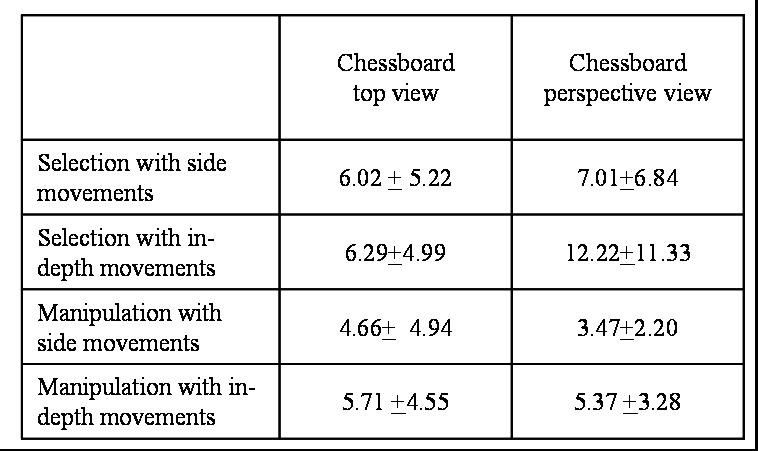
\includegraphics[width=.7\textwidth]{table.jpg}
%\end{table}



\bibliographystyle{sbc}
\bibliography{sbc-template}

\end{document}
